\documentclass[10pt]{article}
\usepackage{graphicx}
\usepackage{float}

\begin{document}
\title{Go Speed Racer()}
\author{Paul D. Camarata}
\date{22 August 2018}

\maketitle
\pagebreak
\begin{abstract}
"People who think they know everything are a great annoyance to those of us who do."
-Isaac Asimov.
\end{abstract}

\section{Introduction}
The purpose of this exploitation project was to gain a better understanding of how a race condition can be used to manipulate something.  Following a guide, I am able to create a vulnerable program using C, which will then be exploited for the purpose of privilege escalation.  All of the work performed on this project is available on github, https://github.com/paulcamarata/CYBR-570.

\section{Part I: Before Coding}
A vulnerable program has been provided for us.  However, the mechanism that this program uses has been fixed in most operating systems.  Since this is the case, we will need to do a something to the operating system prior to execution to get the exploit to work.  

\begin{figure}[H]
\centering
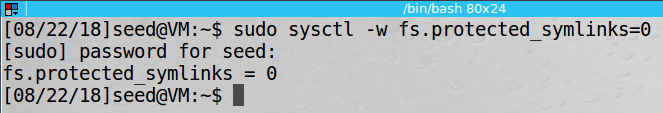
\includegraphics[scale=0.5]{./images/ss01.png}
\caption{OS Tweak}
\label{fig:Code}
\end{figure}

\section{The Code}
The program we are execution is very simple.  The concept is to point to a file, check if we have permission to access the file, and then append a small amount of information to that file.  

\begin{verbatim}
#include <stdio.h>
#include<unistd.h>
int main() {
    char * fn = "/tmp/XYZ";
    char buffer[60];
    FILE *fp;

    /* get user input */
    scanf("%50s", buffer );
    if(!access(fn, W_OK)) {
        fp = fopen(fn, "a+");
        fwrite("\n", sizeof(char), 1, fp);
        fwrite(buffer, sizeof(char), strlen(buffer), fp);
        fclose(fp);
    }

    else printf("No permission \n");
}
\end{verbatim}

\section{The Exploit}
While going through this program, we notice that there is a known issue with the 'access' command.  The concept is that there is a delay between 'access' and 'fopen' that a malicious party can act on.  

\begin{verbatim}
void run(Task *task, int slice) {
    printf("Running task = [%s] [%d] [%d] for %d units.\n",task->name, task->priority, task->burst, slice);
}
\end{verbatim}

\subsection{insert()}
Insert ends up being a very important function for creating the list.  This function is the nuts and bolts for how you create the linked list.  It grabs the current location of the list, inserts the new task at the front of it, and shifts the head of the list.

\begin{verbatim}
void insert(struct node **head, Task *newTask) {
    // add the new task to the list 
    struct node *newNode = malloc(sizeof(struct node));

    newNode->task = newTask;
    newNode->next = *head;
    *head = newNode;
}
\end{verbatim}
\subsection{delete()}
The delete function removes a task from the list.  It does this by tweaking the linking in the list.  If the item is at the start of the list, then it just changes the location of head.  If it is anywhere in the middle, then it finds the previous task and sets its 'next' location to be the item after the deleted task.  This function is intended to be run when a task has fully completed its burst. 

\begin{verbatim}
void delete(struct node **head, Task *task) {
    struct node *temp;
    struct node *prev;

    temp = *head;
    // special case - beginning of list
    if (strcmp(task->name,temp->task->name) == 0) {
        *head = (*head)->next;
    }
    else {
        // interior or last element in the list
        prev = *head;
        temp = temp->next;
        while (strcmp(task->name,temp->task->name) != 0) {
            prev = temp;
            temp = temp->next;
        }

        prev->next = temp->next;
    }
}
\end{verbatim}

\subsection{add()}
The last function provided to us is add().  This function is called from main() and helps setup the task structure that will be required for the insert() function to work properly. 

\begin{verbatim}
void add(char *name, int priority, int burst) {
    // first create the new task
    Task *newTask = (Task *) malloc(sizeof(Task));
    
    newTask->name = name;
    newTask->priority = priority;
    newTask->burst = burst;
	
    // insert the new task into the list of tasks 
    insert(&head, newTask);
}
\end{verbatim}
\section{Part II: My Code}
All code written by me is included in the appendices.  This section is here to walk through my thoughts on how to write the code and reference some of the things actually done.  There were two placeholders provided to me in the sample file, schedule() and pickNextTask().

\subsection{schedule()}
I interpreted this function to be the "How" to run a task.  There are several ways to set this function up, but I opted to utilize recursion.  After talking to another classmate, he explained to me why, in this particular instance, recursion might work, but is not the most optimal way to set this up.  I am able to show that it is capable of working however.  

There are two different paths with my schedule function.  One is used for all programs that run to completion once a task has been chosen.  The other method is for hanlding round robin based scheduling.  The latter ends up being more complicated.

The goal for all schedule functions is to take the selected task, run it for the duration required, and then either update it and place it back in the queue or delete it from the queue once it is done.

\subsection{pickNextTask()}
This function, in my opinion, was more of the "What" to run.  Every time schedule() runs, it makes a call to pickNextTask().  This function then provides a task to be run.  The goal with this function was to step through the list using a pointer, or two, to make a decision on which task is appropriate depending on the scheduling algorithm desired.


\section{Part III: Results}
This section is very straight forward.  First we compile the correct code, per the make file, and then we execute the desired schedule.  All code executes correctly and the programs gracefully exit.


\section{Conclusion}
In conclusion, I think this was an interesting programming project.  I would definitely be interested in a project that dives a bit deeper.  I felt that with the examples presented in class it was impossible to not be able to complete the steps needed to program these applications.  The crazy thing to me is how many people in class complained about how this was some third year programming activity.  I did take one basic C course about 15 years ago, and have not touched the language much since.  I also don't develop for a living, but I am familiar with coding and coding concepts, as I think any modern engineer in a computer based field should be.  I think if you asked me to build the entire program instead of just two functions, the complaints might have had some merit, but since we were just filling in the gaps I thought it was pretty simple once I was able to follow the code.

\pagebreak
\section{Appendix A: FCFS Code}
\begin{verbatim}
void schedule() {

    Task *currentTask = pickNextTask();

    if(!currentTask) {
        exit(0);
    }

    run(currentTask, currentTask->burst);
    delete(&head, currentTask);
    schedule();
}

Task *pickNextTask() {

    struct node *temp;
    temp = head;

    if (!temp){
        printf("Nice job! Teacher, give this student an A.\n");
        exit(0);
    }
    
    while (temp) {
        if(!temp->next) {
            return temp->task;
        }

        temp = temp->next;
    }

    return 0;
}
\end{verbatim}

\pagebreak
\section{Appendix B: SJF Code}
\begin{verbatim}
void schedule() {

    Task *currentTask = pickNextTask();

    if(!currentTask) {
        exit(0);
    }

    run(currentTask, currentTask->burst);
    delete(&head, currentTask);
    schedule();
}

Task *pickNextTask() {

    struct node *temp;
    temp = head;

    if (!temp){
        printf("Nice job! Teacher, give this student an A.\n");
        exit(0);
    }

    int sjf = temp->task->burst;
    Task *chosenTask = temp->task;

    while (temp) {

        if(temp->task->burst <= sjf) {
            sjf = temp->task->burst;
            chosenTask = temp->task;
        }

        if(!temp->next) {
            return chosenTask;
        }

        temp = temp->next;
    }

    return 0;
}
\end{verbatim}

\pagebreak
\section{Appendix C: Priority Code}
\begin{verbatim}
void schedule() {
    
    Task *currentTask = pickNextTask();

    if(currentTask == NULL) {
        exit(0);
    }

    run(currentTask, currentTask->burst);
    delete(&head, currentTask);
    schedule();
}

Task *pickNextTask() {

    struct node *temp;
    temp = head;

    if (!temp){
        printf("Nice job! Teacher, give this student an A.\n");
        exit(0);
    }
 
    int pri = temp->task->priority;
    Task *chosenTask = temp->task;

    while (temp) {
        if(temp->task->priority >= pri) {
            pri = temp->task->priority;
            chosenTask = temp->task;
        }
        if(!temp->next) {
            return chosenTask;
        }
        temp = temp->next;
    }
    return 0;
}
\end{verbatim}

\pagebreak
\section{Appendix D: Round Robin Code}
\begin{verbatim}
void schedule() {
    
    Task *currentTask = pickNextTask();

    if(!currentTask) {
        exit(0);
    }

    if(currentTask->burst > QUANTUM) {
        run(currentTask, QUANTUM);
        currentTask->burst = currentTask->burst - QUANTUM;
        delete(&head, currentTask);
        insert(&head, currentTask);
    } else {
        run(currentTask, currentTask->burst);
        delete(&head, currentTask);
    }
    schedule();
}

Task *pickNextTask() {

    struct node *temp;
    temp = head;

    if (!temp){
        printf("Nice job! Teacher, give this student an A.\n");
        exit(0);
    }
    
    while (temp) {
        if(!temp->next) {
            return temp->task;
        }
        temp = temp->next;
    }

    return 0;
}
\end{verbatim}

\pagebreak
\section{Appendix E: Priority Round Robin Code}
\begin{verbatim}
void schedule() {

    Task *currentTask = pickNextTask();
    
    if(!currentTask) {
        exit(0);
    }
    if(currentTask->burst > QUANTUM) {
        run(currentTask, QUANTUM);
        currentTask->burst = currentTask->burst - QUANTUM;
        delete(&head, currentTask);
        insert(&head, currentTask);
    } else {
        run(currentTask, currentTask->burst);
        delete(&head, currentTask);
    }
    schedule();
}

Task *pickNextTask() {
    
    struct node *temp;
    temp = head;

    if (!temp){
        printf("Nice job! Teacher, give this student an A.\n");
        exit(0);
    }

    int pri = temp->task->priority;
    Task *chosenTask = temp->task;

    while (temp) {
        if(temp->task->priority >= pri) {
            pri = temp->task->priority;
            chosenTask = temp->task;
        }
        if(!temp->next) {
            return chosenTask;
        }
        temp = temp->next;
    }
    return 0;
}
\end{verbatim}

\pagebreak
\begin{thebibliography}{9}
\bibitem{OSConcepts}
Abraham Silberschatz, Peter Baer Galvin, Greg Gagne
\textit{Operating System Concepts}
John Wiley \& Sons Inc. 2018
\end{thebibliography}
\end{document}